%% PNAStmpl.tex
%% Template file to use for PNAS articles prepared in LaTeX
%% Version: Apr 14, 2008


%%%%%%%%%%%%%%%%%%%%%%%%%%%%%%
%% BASIC CLASS FILE 
%% PNAStwo for two column articles is called by default.
%% Uncomment PNASone for single column articles. One column class
%% and style files are available upon request from pnas@nas.edu.
%% (uncomment means get rid of the '%' in front of the command)

%\documentclass{pnasone}
\documentclass{pnastwo}

%%%%%%%%%%%%%%%%%%%%%%%%%%%%%%
%% Changing position of text on physical page:
%% Since not all printers position
%% the printed page in the same place on the physical page,
%% you can change the position yourself here, if you need to:

% \advance\voffset -.5in % Minus dimension will raise the printed page on the 
                         %  physical page; positive dimension will lower it.

%% You may set the dimension to the size that you need.

%%%%%%%%%%%%%%%%%%%%%%%%%%%%%%
%% OPTIONAL GRAPHICS STYLE FILE

%% Requires graphics style file (graphicx.sty), used for inserting
%% .eps files into LaTeX articles.
%% Note that inclusion of .eps files is for your reference only;
%% when submitting to PNAS please submit figures separately.

%% Type into the square brackets the name of the driver program 
%% that you are using. If you don't know, try dvips, which is the
%% most common PC driver, or textures for the Mac. These are the options:

% [dvips], [xdvi], [dvipdf], [dvipdfm], [dvipdfmx], [pdftex], [dvipsone],
% [dviwindo], [emtex], [dviwin], [pctexps], [pctexwin], [pctexhp], [pctex32],
% [truetex], [tcidvi], [vtex], [oztex], [textures], [xetex]

%\usepackage[dvips]{graphicx}

%%%%%%%%%%%%%%%%%%%%%%%%%%%%%%
%% OPTIONAL POSTSCRIPT FONT FILES

%% PostScript font files: You may need to edit the PNASoneF.sty
%% or PNAStwoF.sty file to make the font names match those on your system. 
%% Alternatively, you can leave the font style file commands commented out
%% and typeset your article using the default Computer Modern 
%% fonts (recommended). If accepted, your article will be typeset
%% at PNAS using PostScript fonts.


% Choose PNASoneF for one column; PNAStwoF for two column:
%\usepackage{PNASoneF}
%\usepackage{PNAStwoF}

%%%%%%%%%%%%%%%%%%%%%%%%%%%%%%
%% ADDITIONAL OPTIONAL STYLE FILES

%% The AMS math files are commonly used to gain access to useful features
%% like extended math fonts and math commands.

\usepackage{amssymb,amsfonts,amsmath,amsthm}

%%%%%%%%%%%%%%%%%%%%%%%%%%%%%%
%% OPTIONAL MACRO FILES
%% Insert self-defined macros here.
%% \newcommand definitions are recommended; \def definitions are supported

%\newcommand{\mfrac}[2]{\frac{\displaystyle #1}{\displaystyle #2}}
%\def\s{\sigma}

\def\bc{{\mathcal B}}
\def\btc{{\mathcal{BT}}}

\newcommand{\HC}{\operatorname{Hoch}}
\newcommand{\HH}{\operatorname{HH}}

\newcommand{\CM}[2]{C_*(\Maps(#1 \to #2))}
\newcommand{\CD}[1]{C_*(\Diff(#1))}
\newcommand{\CH}[1]{CH_*(#1)}

\newcommand{\cl}[1]{\underrightarrow{#1}}
\newcommand{\clh}[1]{\underrightarrow{#1}_{{}_{{}_{{}_h}}}}


\newcommand{\Set}{\text{\textbf{Set}}}
\newcommand{\Vect}{\text{\textbf{Vect}}}
\newcommand{\Kom}{\text{\textbf{Kom}}}
\newcommand{\Cat}{\mathcal{C}}

\newcommand{\cell}{\mathfrak{D}}

\newcommand{\into}{\hookrightarrow}
\newcommand{\onto}{\twoheadrightarrow}
\newcommand{\iso}{\cong}
\newcommand{\quism}{\underset{\text{q.i.}}{\simeq}}
\newcommand{\htpy}{\simeq}
\newcommand{\actsOn}{\circlearrowright}
\newcommand{\xto}[1]{\xrightarrow{#1}}
\newcommand{\isoto}{\xto{\iso}}
\newcommand{\quismto}{\xrightarrow[\text{q.i.}]{\iso}}
\newcommand{\diffeoto}{\xrightarrow[\text{diffeo}]{\iso}}
\newcommand{\htpyto}{\xrightarrow[\text{htpy}]{\htpy}}

\newcommand{\directSum}{\oplus}
\newcommand{\DirectSum}{\bigoplus}
\newcommand{\tensor}{\otimes}
\newcommand{\Tensor}{\bigotimes}

\newcommand{\Bord}{\operatorname{Bord}}

\newcommand{\selfarrow}{\ensuremath{\smash{\tikz[baseline]{\clip (0,0.36) rectangle (0.39,-0.16); \draw[->] (0,0.2) .. controls (0.5,0.6) and (0.5,-0.4) .. (0,0);}}}}

\newcommand{\bdy}{\partial}
\newcommand{\compose}{\circ}
\newcommand{\eset}{\emptyset}

\newcommand{\id}{\boldsymbol{1}}

% kw_macros

%!TEX root = ../blob1.tex

%%%%% excerpts from KW's include file of standard macros
%%% (with various new ones added)

\def\z{\mathbb{Z}}
\def\r{\mathbb{R}}
\def\c{\mathbb{C}}
\def\t{\mathbb{T}}
\def\ebb{\mathbb{E}}

\def\k{{\bf k}}

\def\du{\sqcup}
\def\bd{\partial}
\def\sub{\subset}
\def\subeq{\subseteq}
\def\sup{\supset}
%\def\setmin{\smallsetminus}
\def\setmin{\setminus}
\def\ep{\epsilon}
\def\sgl{_\mathrm{gl}}
\def\op{^\mathrm{op}}
\def\deq{\stackrel{\mathrm{def}}{=}}
\def\pd#1#2{\frac{\partial #1}{\partial #2}}
%\def\lf{\overline{\cC}}
\def\lf{\cC}
\def\ot{\otimes}
\def\vphi{\varphi}
\def\inv{^{-1}}
\def\ol{\overline}
\def\BD{BD}

\def\spl{_\pitchfork}


% equations
\newcommand{\eq}[1]{\begin{displaymath}#1\end{displaymath}}
\newcommand{\eqar}[1]{\begin{eqnarray*}#1\end{eqnarray*}}
\newcommand{\eqspl}[1]{\begin{displaymath}\begin{split}#1\end{split}\end{displaymath}}

\DeclareMathOperator*{\colim}{colim}
\DeclareMathOperator*{\hocolim}{hocolim}

\DeclareMathOperator{\most}{most}
\DeclareMathOperator{\rest}{rest}


\DeclareMathOperator{\kone}{cone}


% new theorems

\newtheorem{prop}{Proposition}
\newtheorem{property}[prop]{Property}
\newtheorem{thm}[prop]{Theorem}
\newtheorem{lem}[prop]{Lemma}
\newtheorem{defn}[prop]{Definition}
\newtheorem{axiom}[prop]{Axiom}

\newenvironment{rem}{\noindent\textsl{Remark.}}{}

% \mathrlap -- a horizontal \smash--------------------------------
% For comparison, the existing overlap macros:
% \def\llap#1{\hbox to 0pt{\hss#1}}
% \def\rlap#1{\hbox to 0pt{#1\hss}}
\def\clap#1{\hbox to 0pt{\hss#1\hss}}
\def\mathllap{\mathpalette\mathllapinternal}
\def\mathrlap{\mathpalette\mathrlapinternal}
\def\mathclap{\mathpalette\mathclapinternal}
\def\mathllapinternal#1#2{%
\llap{$\mathsurround=0pt#1{#2}$}}
\def\mathrlapinternal#1#2{%
\rlap{$\mathsurround=0pt#1{#2}$}}
\def\mathclapinternal#1#2{%
\clap{$\mathsurround=0pt#1{#2}$}}

% tricky way to iterate macros over a list
\def\semicolon{;}
\def\applytolist#1{
    \expandafter\def\csname multi#1\endcsname##1{
        \def\multiack{##1}\ifx\multiack\semicolon
            \def\next{\relax}
        \else
            \csname #1\endcsname{##1}
            \def\next{\csname multi#1\endcsname}
        \fi
        \next}
    \csname multi#1\endcsname}

% \def\cA{{\cal A}} for A..Z
\def\calc#1{\expandafter\def\csname c#1\endcsname{{\mathcal #1}}}
\applytolist{calc}QWERTYUIOPLKJHGFDSAZXCVBNM;

% \def\bbA{{\mathbb A}} for A..Z
\def\bbc#1{\expandafter\def\csname bb#1\endcsname{{\mathbb #1}}}
\applytolist{bbc}QWERTYUIOPLKJHGFDSAZXCVBNM;

% \def\bA{{\mathbf A}} for A..Z
\def\bfc#1{\expandafter\def\csname bf#1\endcsname{{\mathbf #1}}}
\applytolist{bfc}QWERTYUIOPLKJHGFDSAZXCVBNM;

% \DeclareMathOperator{\pr}{pr} etc.
\def\declaremathop#1{\expandafter\DeclareMathOperator\csname #1\endcsname{#1}}
\applytolist{declaremathop}{im}{gl}{ev}{coinv}{tr}{rot}{Eq}{obj}{mor}{ob}{Rep}{Tet}{cat}{Maps}{Diff}{Homeo}{sign}{supp}{Nbd}{res}{rad}{Compat};

% \todo, \nn and \noop
\newcommand{\todo}[1]{\textbf{\color[rgb]{.8,.2,.5}\small TODO: #1}}
\def\nn#1{{{\color[rgb]{.2,.5,.6} \small [[#1]]}}}
\long\def\noop#1{}



% references

\newcommand{\arxiv}[1]{\href{http://arxiv.org/abs/#1}{\tt arXiv:\nolinkurl{#1}}}
\newcommand{\doi}[1]{\href{http://dx.doi.org/#1}{{\tt DOI:#1}}}
\newcommand{\euclid}[1]{\href{http://projecteuclid.org/euclid.cmp/#1}{{\tt at Project Euclid: #1}}}
\newcommand{\mathscinet}[1]{\href{http://www.ams.org/mathscinet-getitem?mr=#1}{\tt #1}}
\newcommand{\googlebooks}[1]{(preview at \href{http://books.google.com/books?id=#1}{google books})}



% figures

\newcommand{\mathfig}[2]{\ensuremath{\hspace{-3pt}\begin{array}{c}%
  \raisebox{-2.5pt}{\includegraphics[width=#1\textwidth]{diagrams/#2}}%
\end{array}\hspace{-3pt}}}


% packages

\usepackage{tikz}
\usetikzlibrary{shapes}
\usetikzlibrary{backgrounds}
\usetikzlibrary{decorations,decorations.pathreplacing}
\usetikzlibrary{fit,calc,through}

\usepackage[all,color]{xy}
\SelectTips{cm}{}

\usepackage[pdftex,plainpages=false,hypertexnames=false,pdfpagelabels]{hyperref}

\usepackage{xcolor}
\definecolor{dark-red}{rgb}{0.7,0.25,0.25}
\definecolor{dark-blue}{rgb}{0.15,0.15,0.55}
\definecolor{medium-blue}{rgb}{0,0,0.65}

\hypersetup{
    colorlinks, linkcolor={dark-red},
    citecolor={dark-blue}, urlcolor={medium-blue}
}


%%%%%%%%%%%%%%%%%%%%%%%%%%%%%%
%% Don't type in anything in the following section:
%%%%%%%%%%%%
%% For PNAS Only:
\contributor{Submitted to Proceedings
of the National Academy of Sciences of the United States of America}
%\url{www.pnas.org/cgi/doi/10.1073/pnas.0709640104}
\copyrightyear{2008}
\issuedate{Issue Date}
\volume{Volume}
\issuenumber{Issue Number}
%%%%%%%%%%%%

\begin{document}

%%%%%%%%%%%%%%%%%%%%%%%%%%%%%%


%% For titles, only capitalize the first letter
%% \title{Almost sharp fronts for the surface quasi-geostrophic equation}

\title{Higher categories, colimits, and the blob complex}


%% Enter authors via the \author command.  
%% Use \affil to define affiliations.
%% (Leave no spaces between author name and \affil command)

%% Note that the \thanks{} command has been disabled in favor of
%% a generic, reserved space for PNAS publication footnotes.

%% \author{<author name>
%% \affil{<number>}{<Institution>}} One number for each institution.
%% The same number should be used for authors that
%% are affiliated with the same institution, after the first time
%% only the number is needed, ie, \affil{number}{text}, \affil{number}{}
%% Then, before last author ...
%% \and
%% \author{<author name>
%% \affil{<number>}{}}

%% For example, assuming Garcia and Sonnery are both affiliated with
%% Universidad de Murcia:
%% \author{Roberta Graff\affil{1}{University of Cambridge, Cambridge,
%% United Kingdom},
%% Javier de Ruiz Garcia\affil{2}{Universidad de Murcia, Bioquimica y Biologia
%% Molecular, Murcia, Spain}, \and Franklin Sonnery\affil{2}{}}

\author{Scott Morrison\affil{1}{Miller Institute for Basic Research, UC Berkeley, CA 94704, USA} 
\and Kevin Walker\affil{2}{Microsoft Station Q, 2243 CNSI Building, UC Santa Barbara, CA 93106, USA}}

\contributor{Submitted to Proceedings of the National Academy of Sciences
of the United States of America}

%% The \maketitle command is necessary to build the title page.
\maketitle

%%%%%%%%%%%%%%%%%%%%%%%%%%%%%%%%%%%%%%%%%%%%%%%%%%%%%%%%%%%%%%%%
\begin{article}

\begin{abstract}
We summarize our axioms for higher categories, and describe the ``blob complex". 
Fixing an $n$-category $\cC$, the blob complex associates a chain complex $\bc_*(W;\cC)$ to any $n$-manifold $W$. 
The $0$-th homology of this chain complex recovers the usual topological quantum field theory invariants of $W$. 
The higher homology groups should be viewed as generalizations of Hochschild homology (indeed, when $W=S^1$ they coincide). 
The blob complex has a very natural definition in terms of homotopy colimits along decompositions of the manifold $W$. 
We outline the important properties of the blob complex, and sketch the proof of a generalization of 
Deligne's conjecture on Hochschild cohomology and the little discs operad to higher dimensions.
\end{abstract}


%% When adding keywords, separate each term with a straight line: |
\keywords{n-categories | topological quantum field theory | hochschild homology}

%% Optional for entering abbreviations, separate the abbreviation from
%% its definition with a comma, separate each pair with a semicolon:
%% for example:
%% \abbreviations{SAM, self-assembled monolayer; OTS,
%% octadecyltrichlorosilane}

% \abbreviations{TQFT, topological quantum field theory}

%% The first letter of the article should be drop cap: \dropcap{}
%\dropcap{I}n this article we study the evolution of ''almost-sharp'' fronts

%% Enter the text of your article beginning here and ending before
%% \begin{acknowledgements}
%% Section head commands for your reference:
%% \section{}
%% \subsection{}
%% \subsubsection{}

\dropcap{T}he aim of this paper is to describe a derived category analogue of topological quantum field theories.

For our purposes, an $n{+}1$-dimensional TQFT is a locally defined system of
invariants of manifolds of dimensions 0 through $n{+}1$. In particular,
the TQFT invariant $A(Y)$ of a closed $k$-manifold $Y$ is a linear $(n{-}k)$-category.
If $Y$ has boundary then $A(Y)$ is a collection of $(n{-}k)$-categories which afford
a representation of the $(n{-}k{+}1)$-category $A(\bd Y)$.
(See \cite{1009.5025} and \cite{kw:tqft};
for a more homotopy-theoretic point of view see \cite{0905.0465}.)

We now comment on some particular values of $k$ above.
A linear 0-category is a vector space, and a representation
of a vector space is an element of the dual space.
Thus a TQFT assigns to each closed $n$-manifold $Y$ a vector space $A(Y)$,
and to each $(n{+}1)$-manifold $W$ an element of $A(\bd W)^*$.
For the remainder of this paper we will in fact be interested in so-called $(n{+}\epsilon)$-dimensional
TQFTs, which are slightly weaker structures in that they assign 
invariants to mapping cylinders of homeomorphisms between $n$-manifolds, but not to general $(n{+}1)$-manifolds.

When $k=n{-}1$ we have a linear 1-category $A(S)$ for each $(n{-}1)$-manifold $S$,
and a representation of $A(\bd Y)$ for each $n$-manifold $Y$.
The TQFT gluing rule in dimension $n$ states that
$A(Y_1\cup_S Y_2) \cong A(Y_1) \ot_{A(S)} A(Y_2)$,
where $Y_1$ and $Y_2$ are $n$-manifolds with common boundary $S$.

When $k=0$ we have an $n$-category $A(pt)$.
This can be thought of as the local part of the TQFT, and the full TQFT can be reconstructed from $A(pt)$
via colimits (see below).

We call a TQFT semisimple if $A(S)$ is a semisimple 1-category for all $(n{-}1)$-manifolds $S$
and $A(Y)$ is a finite-dimensional vector space for all $n$-manifolds $Y$.
Examples of semisimple TQFTs include Witten-Reshetikhin-Turaev theories, 
Turaev-Viro theories, and Dijkgraaf-Witten theories.
These can all be given satisfactory accounts in the framework outlined above.
(The WRT invariants need to be reinterpreted as $3{+}1$-dimensional theories with only a weak 
dependence on interiors in order to be
extended all the way down to dimension 0.)

For other non-semisimple TQFT-like invariants, however, the above framework seems to be inadequate.
For example, the gluing rule for 3-manifolds in Ozsv\'ath-Szab\'o/Seiberg-Witten theory
involves a tensor product over an $A_\infty$ 1-category associated to 2-manifolds \cite{1003.0598,1005.1248}.
Long exact sequences are important computational tools in these theories,
and also in Khovanov homology, but the colimit construction breaks exactness.
For these reasons and others, it is desirable to 
extend to above framework to incorporate ideas from derived categories.

One approach to such a generalization might be to simply define a
TQFT via its gluing formulas, replacing tensor products with
derived tensor products (c.f. \cite{1011.1958}).
However, it is probably difficult to prove
the invariance of such a definition, as the object associated to a manifold
will a priori depend on the explicit presentation used to apply the gluing formulas.
We instead give a manifestly invariant construction, and
deduce from it the gluing formulas based on $A_\infty$ tensor products.

This paper is organized as follows.
We first give an account of our version of $n$-categories.
According to our definition, $n$-categories are, among other things,
functorial invariants of $k$-balls, $0\le k \le n$, which behave well with respect to gluing.
We then show how to extend an $n$-category from balls to arbitrary $k$-manifolds,
using colimits and homotopy colimits.
This extension, which we call the blob complex, has as $0$-th homology the usual TQFT invariant.
(The name comes from the ``blobs" which feature prominently
in a concrete version of the homotopy colimit.)
We then review some basic properties of the blob complex, and finish by showing how it
yields a higher categorical and higher dimensional generalization of Deligne's
conjecture on Hochschild cochains and the little 2-disks operad.

At several points we only sketch an argument briefly; full details can be found in \cite{1009.5025}. 
In this paper we attempt to give a clear view of the big picture without getting 
bogged down in technical details.


\section{Definitions}
\subsection{$n$-categories} \mbox{}

In this section we give a definition of $n$-categories designed to work well with TQFTs.
The main idea is to base the definition on actual balls, rather combinatorial models of them.
This has the advantages of avoiding a proliferation of coherency axioms and building in a strong
version of duality from the start.


%\nn{maybe say something about goals: well-suited to TQFTs; avoid proliferation of coherency axioms;
%non-recursive (n-cats not defined n terms of (n-1)-cats; easy to show that the motivating
%examples satisfy the axioms; strong duality; both plain and infty case;
%(?) easy to see that axioms are correct, in the sense of nothing missing (need
%to say this better if we keep it)}
%
%\nn{maybe: the typical n-cat definition tries to do two things at once: (1) give a list of basic properties
%which are weak enough to include the basic examples and strong enough to support the proofs
%of the main theorems; and (2) specify a minimal set of generators and/or axioms.
%We separate these two tasks, and address only the first, which becomes much easier when not burdened by the second.
%More specifically, life is easier when working with maximal, rather than minimal, collections of axioms.}

Of course, there are currently many interesting alternative notions of $n$-category.
We note that our $n$-categories are both more and less general
than the ``fully dualizable" ones which play a prominent role in \cite{0905.0465}.
They are more general in that we make no duality assumptions in the top dimension $n{+}1$.
They are less general in that we impose stronger duality requirements in dimensions 0 through $n$.
Thus our $n$-categories correspond to $(n{+}\epsilon)$-dimensional {\it unoriented} or {\it oriented} TQFTs, while
Lurie's (fully dualizable) $n$-categories correspond to $(n{+}1)$-dimensional {\it framed} TQFTs.

We will define two variations simultaneously,  as all but one of the axioms are identical in the two cases.
These variations are ``ordinary $n$-categories", where homeomorphisms fixing the boundary
act trivially on the sets associated to $n$-balls
(and these sets are usually vector spaces or more generally modules over a commutative ring)
and ``$A_\infty$ $n$-categories",  where there is a homotopy action of
$k$-parameter families of homeomorphisms on these sets
(which are usually chain complexes or topological spaces).

There are five basic ingredients 
\cite{life-of-brian} of an $n$-category definition:
$k$-morphisms (for $0\le k \le n$), domain and range, composition,
identity morphisms, and special behavior in dimension $n$ (e.g. enrichment
in some auxiliary category, or strict associativity instead of weak associativity).
We will treat each of these in turn.

To motivate our morphism axiom, consider the venerable notion of the Moore loop space
\cite[\S 2.2]{MR505692}.
In the standard definition of a loop space, loops are always parameterized by the unit interval $I = [0,1]$,
so composition of loops requires a reparameterization $I\cup I \cong I$, and this leads to a proliferation
of higher associativity relations.
While this proliferation is manageable for 1-categories (and indeed leads to an elegant theory
of Stasheff polyhedra and $A_\infty$ categories), it becomes undesirably complex for higher categories.
In a Moore loop space, we have a separate space $\Omega_r$ for each interval $[0,r]$, and a 
{\it strictly associative} composition $\Omega_r\times \Omega_s\to \Omega_{r+s}$.
Thus we can have the simplicity of strict associativity in exchange for more morphisms.
We wish to imitate this strategy in higher categories.
Because we are mainly interested in the case of pivotal $n$-categories, we replace the intervals $[0,r]$ not with
a product of $k$ intervals (c.f. \cite{ulrike-tillmann-2008,0909.2212}) but rather with any $k$-ball, that is, 
any $k$-manifold which is homeomorphic
to the standard $k$-ball $B^k$.

By default our balls are unoriented,
but it is useful at times to vary this,
for example by considering oriented or Spin balls.
We can also consider more exotic structures, such as balls with a map to some target space,
or equipped with $m$ independent vector fields.
(The latter structure would model $n$-categories with less duality than we usually assume.)

\begin{axiom}[Morphisms]
\label{axiom:morphisms}
For each $0 \le k \le n$, we have a functor $\cC_k$ from 
the category of $k$-balls and 
homeomorphisms to the category of sets and bijections.
\end{axiom}

Note that the functoriality in the above axiom allows us to operate via
homeomorphisms which are not the identity on the boundary of the $k$-ball.
The action of these homeomorphisms gives the pivotal structure.
For this reason we don't subdivide the boundary of a morphism
into domain and range in the next axiom --- the duality operations can convert between domain and range.

Later we inductively define an extension of the functors $\cC_k$ to functors $\cl{\cC}_k$ 
defined on arbitrary manifolds. 
We need  these functors for $k$-spheres, for $k<n$, for the next axiom.

\begin{axiom}[Boundaries]\label{nca-boundary}
For each $k$-ball $X$, we have a map of sets $\bd: \cC_k(X)\to \cl{\cC}_{k-1}(\bd X)$.
These maps, for various $X$, comprise a natural transformation of functors.
\end{axiom}

For $c\in \cl{\cC}_{k-1}(\bd X)$ we define $\cC_k(X; c) = \bd^{-1}(c)$.

Many of the examples we are interested in are enriched in some auxiliary category $\cS$
(e.g. vector spaces or rings, or, in the $A_\infty$ case, chain complexes or topological spaces).
This means that in the top dimension $k=n$ the sets $\cC_n(X; c)$ have the structure
of an object of $\cS$, and all of the structure maps of the category (above and below) are
compatible with the $\cS$ structure on $\cC_n(X; c)$.


Given two hemispheres (a ``domain" and ``range") that agree on the equator, we need to be able to 
assemble them into a boundary value of the entire sphere.

\begin{lem}
\label{lem:domain-and-range}
Let $S = B_1 \cup_E B_2$, where $S$ is a $k{-}1$-sphere $(1\le k\le n)$,
$B_i$ is a $k{-}1$-ball, and $E = B_1\cap B_2$ is a $k{-}2$-sphere (Figure \ref{blah3}).
Let $\cC(B_1) \times_{\cl{\cC}(E)} \cC(B_2)$ denote the fibered product of the 
two maps $\bd: \cC(B_i)\to \cl{\cC}(E)$.
Then we have an injective map
\[
	\gl_E : \cC(B_1) \times_{\cl{\cC}(E)} \cC(B_2) \into \cl{\cC}(S)
\]
which is natural with respect to the actions of homeomorphisms.
%(When $k=1$ we stipulate that $\cl{\cC}(E)$ is a point, so that the above fibered product
%becomes a normal product.)
\end{lem}

If $\bdy B = S$, we denote $\bdy^{-1}(\im(\gl_E))$ by $\cC(B)_E$.

\begin{axiom}[Gluing]
\label{axiom:composition}
Let $B = B_1 \cup_Y B_2$, where $B$, $B_1$ and $B_2$ are $k$-balls ($0\le k\le n$)
and $Y = B_1\cap B_2$ is a $k{-}1$-ball (Figure \ref{blah5}).
Let $E = \bd Y$, which is a $k{-}2$-sphere.
%Note that each of $B$, $B_1$ and $B_2$ has its boundary split into two $k{-}1$-balls by $E$.
We have restriction maps $\cC(B_i)_E \to \cC(Y)$.
Let $\cC(B_1)_E \times_{\cC(Y)} \cC(B_2)_E$ denote the fibered product of these two maps. 
We have a map
\[
	\gl_Y : \cC(B_1)_E \times_{\cC(Y)} \cC(B_2)_E \to \cC(B)_E
\]
which is natural with respect to the actions of homeomorphisms, and also compatible with restrictions
to the intersection of the boundaries of $B$ and $B_i$.
If $k < n$,
or if $k=n$ and we are in the $A_\infty$ case, 
we require that $\gl_Y$ is injective.
(For $k=n$ in the ordinary $n$-category case, see Axiom \ref{axiom:extended-isotopies}.)
\end{axiom}

\begin{axiom}[Strict associativity] \label{nca-assoc}\label{axiom:associativity}
The gluing maps above are strictly associative.
Given any decomposition of a ball $B$ into smaller balls
$$\bigsqcup B_i \to B,$$ 
any sequence of gluings (where all the intermediate steps are also disjoint unions of balls) yields the same result.
\end{axiom}
%This axiom is only reasonable because the definition assigns a set to every ball; 
%any identifications would limit the extent to which we can demand associativity.
%%%% KW: It took me quite a while figure out what you [or I??] meant by the above, so I'm attempting a rewrite.
Note that even though our $n$-categories are ``weak" in the traditional sense, we can require
strict associativity because we have more morphisms (cf.\ discussion of Moore loops above).

For the next axiom, a \emph{pinched product} is a map locally modeled on a degeneracy map between simplices.
\begin{axiom}[Product (identity) morphisms]
\label{axiom:product}
For each pinched product $\pi:E\to X$, with $X$ a $k$-ball and $E$ a $k{+}m$-ball ($m\ge 1$),
there is a map $\pi^*:\cC(X)\to \cC(E)$.
These maps must be
\begin{enumerate}
\item natural with respect to maps of pinched products,
\item functorial with respect to composition of pinched products, 
\item compatible with gluing and restriction of pinched products.
\end{enumerate}

%%% begin noop %%%
% this was the original list of conditions, which I've replaced with the much terser list above -S
\noop{
These maps must satisfy the following conditions.
\begin{enumerate}
\item
If $\pi:E\to X$ and $\pi':E'\to X'$ are pinched products, and
if $f:X\to X'$ and $\tilde{f}:E \to E'$ are maps such that the diagram
\[ \xymatrix{
	E \ar[r]^{\tilde{f}} \ar[d]_{\pi} & E' \ar[d]^{\pi'} \\
	X \ar[r]^{f} & X'
} \]
commutes, then we have 
\[
	\pi'^*\circ f = \tilde{f}\circ \pi^*.
\]
\item
Product morphisms are compatible with gluing.
Let $\pi:E\to X$, $\pi_1:E_1\to X_1$, and $\pi_2:E_2\to X_2$ 
be pinched products with $E = E_1\cup E_2$.
Let $a\in \cC(X)$, and let $a_i$ denote the restriction of $a$ to $X_i\subset X$.
Then 
\[
	\pi^*(a) = \pi_1^*(a_1)\bullet \pi_2^*(a_2) .
\]
\item
Product morphisms are associative.
If $\pi:E\to X$ and $\rho:D\to E$ are pinched products then
\[
	\rho^*\circ\pi^* = (\pi\circ\rho)^* .
\]
\item
Product morphisms are compatible with restriction.
If we have a commutative diagram
\[ \xymatrix{
	D \ar@{^(->}[r] \ar[d]_{\rho} & E \ar[d]^{\pi} \\
	Y \ar@{^(->}[r] & X
} \]
such that $\rho$ and $\pi$ are pinched products, then
\[
	\res_D\circ\pi^* = \rho^*\circ\res_Y .
\]
\end{enumerate}
} %%% end \noop %%%
\end{axiom}

To state the next axiom we need the notion of {\it collar maps} on $k$-morphisms.
Let $X$ be a $k$-ball and $Y\subset\bd X$ be a $(k{-}1)$-ball.
Let $J$ be a 1-ball.
Let $Y\times_p J$ denote $Y\times J$ pinched along $(\bd Y)\times J$.
A collar map is an instance of the composition
\[
	\cC(X) \to \cC(X\cup_Y (Y\times_p J)) \to \cC(X) ,
\]
where the first arrow is gluing with a product morphism on $Y\times_p J$ and
the second is induced by a homeomorphism from $X\cup_Y (Y\times_p J)$ to $X$ which restricts
to the identity on the boundary.


\begin{axiom}[\textup{\textbf{[for ordinary  $n$-categories]}} Extended isotopy invariance in dimension $n$.]
\label{axiom:extended-isotopies}
Let $X$ be an $n$-ball and $f: X\to X$ be a homeomorphism which restricts
to the identity on $\bd X$ and isotopic (rel boundary) to the identity.
Then $f$ acts trivially on $\cC(X)$.
In addition, collar maps act trivially on $\cC(X)$.
\end{axiom}

\smallskip

For $A_\infty$ $n$-categories, we replace
isotopy invariance with the requirement that families of homeomorphisms act.
For the moment, assume that our $n$-morphisms are enriched over chain complexes.
Let $\Homeo_\bd(X)$ denote homeomorphisms of $X$ which fix $\bd X$ and
$C_*(\Homeo_\bd(X))$ denote the singular chains on this space.


\begin{axiom}[\textup{\textbf{[for $A_\infty$ $n$-categories]}} Families of homeomorphisms act in dimension $n$.]
\label{axiom:families}
For each $n$-ball $X$ and each $c\in \cl{\cC}(\bd X)$ we have a map of chain complexes
\[
	C_*(\Homeo_\bd(X))\tensor \cC(X; c) \to \cC(X; c) .
\]
These action maps are required to restrict to the usual action of homeomorphisms on $C_0$, be associative up to homotopy,
and also be compatible with composition (gluing) in the sense that
a diagram like the one in Theorem \ref{thm:CH} commutes.
\end{axiom}

\subsection{Example (the fundamental $n$-groupoid)} \mbox{}
We will define $\pi_{\le n}(T)$, the fundamental $n$-groupoid of a topological space $T$.
When $X$ is a $k$-ball with $k<n$, define $\pi_{\le n}(T)(X)$
to be the set of continuous maps from $X$ to $T$.
When $X$ is an $n$-ball, define $\pi_{\le n}(T)(X)$ to be homotopy classes (rel boundary) of such maps.
Define boundary restrictions and gluing in the obvious way.
If $\rho:E\to X$ is a pinched product and $f:X\to T$ is a $k$-morphism,
define the product morphism $\rho^*(f)$ to be $f\circ\rho$.

We can also define an $A_\infty$ version $\pi_{\le n}^\infty(T)$ of the fundamental $n$-groupoid.
For $X$ an $n$-ball define $\pi_{\le n}^\infty(T)(X)$ to be the space of all maps from $X$ to $T$
(if we are enriching over spaces) or the singular chains on that space (if we are enriching over chain complexes).


\subsection{Example (string diagrams)} \mbox{}
Fix a ``traditional" pivotal $n$-category $C$ (e.g.\ a pivotal 2-category).
Let $X$ be a $k$-ball and define $\cS_C(X)$ to be the set of $C$ string diagrams drawn on $X$;
that is, certain cell complexes embedded in $X$, with the codimension-$j$ cells labeled by $j$-morphisms of $C$.
If $X$ is an $n$-ball, identify two such string diagrams if they evaluate to the same $n$-morphism of $C$.
Boundary restrictions and gluing are again straightforward to define.
Define product morphisms via product cell decompositions.

\subsection{Example (bordism)} \mbox{}
When $X$ is a $k$-ball with $k<n$, $\Bord^n(X)$ is the set of all $k$-dimensional
submanifolds $W$ in $X\times \bbR^\infty$ which project to $X$ transversely
to $\bd X$.
For an $n$-ball $X$ define $\Bord^n(X)$ to be homeomorphism classes rel boundary of such $n$-dimensional submanifolds.

There is an $A_\infty$ analogue enriched in topological spaces, where at the top level we take 
all such submanifolds, rather than homeomorphism classes. 
For each fixed $\bdy W \subset \bdy X \times \bbR^\infty$, we 
topologize the set of submanifolds by ambient isotopy rel boundary.

\subsection{The blob complex}
\subsubsection{Decompositions of manifolds}
Our description of an $n$-category associates data to each $k$-ball for $k\leq n$. In order to define invariants of $n$-manifolds, we will need a class of decompositions of manifolds into balls. We present one choice here, but alternatives of varying degrees of generality exist, for example handle decompositions or piecewise-linear CW-complexes \cite{1009.4227}.

A \emph{ball decomposition} of a $k$-manifold $W$ is a 
sequence of gluings $M_0\to M_1\to\cdots\to M_m = W$ such that $M_0$ is a disjoint union of balls
$\du_a X_a$ and each $M_i$ is a manifold.
If $X_a$ is some component of $M_0$, its image in $W$ need not be a ball; $\bd X_a$ may have been glued to itself.
A {\it permissible decomposition} of $W$ is a map
\[
	\coprod_a X_a \to W,
\]
which can be completed to a ball decomposition $\du_a X_a = M_0\to\cdots\to M_m = W$.
A permissible decomposition is weaker than a ball decomposition; we forget the order in which the balls
are glued up to yield $W$, and just require that there is some non-pathological way to do this. 

Given permissible decompositions $x = \{X_a\}$ and $y = \{Y_b\}$ of $W$, we say that $x$ is a refinement
of $y$, or write $x \le y$, if there is a ball decomposition $\du_a X_a = M_0\to\cdots\to M_m = W$
with $\du_b Y_b = M_i$ for some $i$.

\begin{defn}
The poset $\cell(W)$ has objects the permissible decompositions of $W$, 
and a unique morphism from $x$ to $y$ if and only if $x$ is a refinement of $y$.
See Figure \ref{partofJfig} for an example.
\end{defn}

This poset in fact has more structure, since we can glue together permissible decompositions of 
$W_1$ and $W_2$ to obtain a permissible decomposition of $W_1 \sqcup W_2$. 

An $n$-category $\cC$ determines 
a functor $\psi_{\cC;W}$ from $\cell(W)$ to the category of sets 
(possibly with additional structure if $k=n$).
Each $k$-ball $X$ of a decomposition $y$ of $W$ has its boundary decomposed into $k{-}1$-manifolds,
and there is a subset $\cC(X)\spl \subset \cC(X)$ of morphisms whose boundaries
are splittable along this decomposition.

\begin{defn}
Define the functor $\psi_{\cC;W} : \cell(W) \to \Set$ as follows.
For a decomposition $x = \bigsqcup_a X_a$ in $\cell(W)$, $\psi_{\cC;W}(x)$ is the subset
\begin{equation*}
%\label{eq:psi-C}
	\psi_{\cC;W}(x) \subset \prod_a \cC(X_a)\spl
\end{equation*}
where the restrictions to the various pieces of shared boundaries amongst the balls
$X_a$ all agree (similar to a fibered product). 
When $k=n$, the ``subset" and ``product" in the above formula should be 
interpreted in the appropriate enriching category.
If $x$ is a refinement of $y$, the map $\psi_{\cC;W}(x) \to \psi_{\cC;W}(y)$ is given by the composition maps of $\cC$.
\end{defn}

%We will use the term ``field on $W$" to refer to a point of this functor,
%that is, a permissible decomposition $x$ of $W$ together with an element of $\psi_{\cC;W}(x)$.


\subsubsection{Colimits}
Recall that our definition of an $n$-category is essentially a collection of functors
defined on the categories of homeomorphisms of $k$-balls
for $k \leq n$ satisfying certain axioms. 
It is natural to hope to extend such functors to the 
larger categories of all $k$-manifolds (again, with homeomorphisms). 
In fact, the axioms stated above already require such an extension to $k$-spheres for $k<n$.

The natural construction achieving this is a colimit along the poset of permissible decompositions.
Given an ordinary $n$-category $\cC$, 
we will denote its extension to all manifolds by $\cl{\cC}$. On a $k$-manifold $W$, with $k \leq n$, 
this is defined to be the colimit along $\cell(W)$ of the functor $\psi_{\cC;W}$. 
Note that Axioms \ref{axiom:composition} and \ref{axiom:associativity} 
imply that $\cl{\cC}(X)  \iso \cC(X)$ when $X$ is a $k$-ball with $k<n$. 
Suppose that $\cC$ is enriched in vector spaces: this means that given boundary conditions $c \in \cl{\cC}(\bdy X)$, for $X$ an $n$-ball, 
the set $\cC(X;c)$ is a vector space. 
In this case, for $W$ an arbitrary $n$-manifold and $c \in \cl{\cC}(\bdy W)$,
the set $\cl{\cC}(W;c) = \bdy^{-1} (c)$ inherits the structure of a vector space. 
These are the usual TQFT skein module invariants on $n$-manifolds.

We can now give a straightforward but rather abstract definition of the blob complex of an $n$-manifold $W$
with coefficients in the $n$-category $\cC$ as the {\it homotopy} colimit along $\cell(W)$
of the functor $\psi_{\cC; W}$ described above. We write this as $\clh{\cC}(W)$.

An explicit realization of the homotopy colimit is provided by the simplices of the 
functor $\psi_{\cC; W}$. That is, $$\clh{\cC}(W) = \DirectSum_{\bar{x}} \psi_{\cC; W}(x_0)[m],$$ 
where $\bar{x} = x_0 \leq \cdots \leq x_m$ is a simplex in $\cell(W)$. 
The differential acts on $(\bar{x},a)$ (here $a \in \psi_{\cC; W}(x_0)$) as
$$\bdy (\bar{x},a) = (\bar{x}, \bdy a) + (-1)^{\deg a} \left( (d_0 \bar{x}, g(a)) + \sum_{i=1}^m (-1)^i (d_i \bar{x}, a) \right)$$
where $g$ is the gluing map from $x_0$ to $x_1$, and $d_i \bar{x}$ denotes the $i$-th face of the simplex $\bar{x}$.

Alternatively, we can take advantage of the product structure on $\cell(W)$ to realize the 
homotopy colimit via the cone-product polyhedra in $\cell(W)$. 
A cone-product polyhedra is obtained from a point by successively taking the cone or taking the 
product with another cone-product polyhedron. Just as simplices correspond to linear directed graphs, 
cone-product polyheda correspond to directed trees: taking cone adds a new root before the existing root, 
and taking product identifies the roots of several trees. 
The ``local homotopy colimit" is then defined according to the same formula as above, but with $\bar{x}$ a cone-product polyhedron in $\cell(W)$. 
We further require that all (compositions of) morphisms in a directed tree are not expressible as a product.
The differential acts on $(\bar{x},a)$ both on $a$ and on $\bar{x}$, applying the appropriate gluing map to $a$ when required.
A Eilenberg-Zilber subdivision argument shows this is the same as the usual realization. 

%When $\cC$ is a topological $n$-category,
%the flexibility available in the construction of a homotopy colimit allows
%us to give a much more explicit description of the blob complex which we'll write as $\bc_*(W; \cC)$.
%\todo{either need to explain why this is the same, or significantly rewrite this section}
When $\cC$ is the ordinary $n$-category based on string diagrams for a traditional
$n$-category $C$,
one can show \cite{1009.5025} that the above two constructions of the homotopy colimit
are equivalent to the more concrete construction which we describe next, and which we denote $\bc_*(W; \cC)$.
Roughly speaking, the generators of $\bc_k(W; \cC)$ are string diagrams on $W$ together with
a configuration of $k$ balls (or ``blobs") in $W$ whose interiors are pairwise disjoint or nested.
The restriction of the string diagram to innermost blobs is required to be ``null" in the sense that
it evaluates to a zero $n$-morphism of $C$.
The next few paragraphs describe this in more detail.

We will call a string diagram on a manifold a ``field".
(See \cite{1009.5025} for a more general notion of field.)

We say a collection of balls $\{B_i\}$ in a manifold $W$ is \emph{permissible}
if there exists a permissible decomposition $M_0\to\cdots\to M_m = W$ such that
each $B_i$ appears as a connected component of one of the $M_j$. 
Note that this forces the balls to be pairwise either disjoint or nested. 
Such a collection of balls cuts $W$ into pieces, the connected components of $W \setminus \bigcup \bdy B_i$. 
These pieces need not be manifolds, 
but they can be further subdivided into pieces which are manifolds
and which fit into a permissible decomposition of $W$.

The $k$-blob group $\bc_k(W; \cC)$ is generated by the $k$-blob diagrams. 
A $k$-blob diagram consists of
\begin{itemize}
	\item a permissible collection of $k$ embedded balls, and
	\item a linear combination $s$ of string diagrams on $W$,
\end{itemize}
such that
\begin{itemize}
	\item there is a permissible decomposition of $W$, compatible with the $k$ blobs, such that
	$s$ is the result of gluing together linear combinations of fields $s_i$ on the initial pieces $X_i$ of the decomposition
	(for fixed restrictions to the boundaries of the pieces),
	\item the $s_i$'s corresponding to innermost blobs evaluate to zero in $\cC$, and
	\item the $s_i$'s corresponding to the other pieces are single fields (linear combinations with only one term).
\end{itemize}
%that for any innermost blob $B$, the field on $B$ goes to zero under the gluing map from $\cC$. 
We call such linear combinations which evaluate to zero on a blob $B$ a ``null field on $B$".
% could maybe say something here like "if blobs have nice complements then this is just...."

The differential acts on a $k$-blob diagram by summing over ways to forget one of the $k$ blobs, with alternating signs.

We now spell this out for some small values of $k$. 
For $k=0$, the $0$-blob group is simply linear combinations of fields (string diagrams) on $W$. 
For $k=1$, a generator consists of a field on $W$ and a ball, such that the restriction of the field to that ball is a null field. 
The differential simply forgets the ball. 
Thus we see that $H_0$ of the blob complex is the quotient of fields by fields which are null on some ball.

For $k=2$, we have a two types of generators; they each consists of a field $f$ on $W$, and two balls $B_1$ and $B_2$. 
In the first case, the balls are disjoint, and $f$ restricted to either of the $B_i$ is a null field. 
In the second case, the balls are properly nested, say $B_1 \subset B_2$, and $f$ restricted to $B_1$ is null. 
Note that this implies that $f$ restricted to $B_2$ is also null, by the associativity of the gluing operation. 
This ensures that the differential is well-defined.

\section{Properties of the blob complex}
\subsection{Formal properties}
\label{sec:properties}
The blob complex enjoys the following list of formal properties. The first three are immediate from the definitions.

\begin{property}[Functoriality]
\label{property:functoriality}%
The blob complex is functorial with respect to homeomorphisms.
That is, 
for a fixed $n$-category $\cC$, the association
\begin{equation*}
X \mapsto \bc_*(X; \cC)
\end{equation*}
is a functor from $n$-manifolds and homeomorphisms between them to chain 
complexes and isomorphisms between them.
\end{property}
As a consequence, there is an action of $\Homeo(X)$ on the chain complex $\bc_*(X; \cC)$; 
this action is extended to all of $C_*(\Homeo(X))$ in Theorem \ref{thm:CH} below.

\begin{property}[Disjoint union]
\label{property:disjoint-union}
The blob complex of a disjoint union is naturally isomorphic to the tensor product of the blob complexes.
\begin{equation*}
\bc_*(X_1 \du X_2) \iso \bc_*(X_1) \tensor \bc_*(X_2)
\end{equation*}
\end{property}

If an $n$-manifold $X$ contains $Y \sqcup Y^\text{op}$ (we allow $Y = \eset$) as a codimension $0$ submanifold of its boundary, 
write $X \bigcup_{Y}\selfarrow$ for the manifold obtained by gluing together $Y$ and $Y^\text{op}$.
\begin{property}[Gluing map]
\label{property:gluing-map}%
%If $X_1$ and $X_2$ are $n$-manifolds, with $Y$ a codimension $0$-submanifold of $\bdy X_1$, and $Y^{\text{op}}$ a codimension $0$-submanifold of $\bdy X_2$, there is a chain map
%\begin{equation*}
%\gl_Y: \bc_*(X_1) \tensor \bc_*(X_2) \to \bc_*(X_1 \cup_Y X_2).
%\end{equation*}
Given a gluing $X \to X \bigcup_{Y}\selfarrow$, there is
a map
\[
	\bc_*(X) \to \bc_*(X \bigcup_{Y}\selfarrow),
\]
natural with respect to homeomorphisms, and associative with respect to iterated gluings.
\end{property}

\begin{property}[Contractibility]
\label{property:contractibility}%
The blob complex on an $n$-ball is contractible in the sense 
that it is homotopic to its $0$-th homology, and this is just the vector space associated to the ball by the $n$-category.
\begin{equation*}
\xymatrix{\bc_*(B^n;\cC) \ar[r]^(0.4){\htpy} & H_0(\bc_*(B^n;\cC)) \ar[r]^(0.6)\iso & \cC(B^n)}
\end{equation*}
\end{property}
%\nn{maybe should say something about the $A_\infty$ case}

\begin{proof}(Sketch)
For $k\ge 1$, the contracting homotopy sends a $k$-blob diagram to the $(k{+}1)$-blob diagram
obtained by adding an outer $(k{+}1)$-st blob consisting of all $B^n$.
For $k=0$ we choose a splitting $s: H_0(\bc_*(B^n)) \to \bc_0(B^n)$ and send 
$x\in \bc_0(B^n)$ to $x - s([x])$, where $[x]$ denotes the image of $x$ in $H_0(\bc_*(B^n))$.
\end{proof}

If $\cC$ is an $A_\infty$ $n$-category then $\bc_*(B^n;\cC)$ is still homotopy equivalent to $\cC(B^n)$,
but this is no longer concentrated in degree zero.

\subsection{Specializations}
\label{sec:specializations}

The blob complex has several important special cases.

\begin{thm}[Skein modules]
\label{thm:skein-modules}
Suppose $\cC$ is an ordinary $n$-category.
The $0$-th blob homology of $X$ is the usual 
(dual) TQFT Hilbert space (a.k.a.\ skein module) associated to $X$
by $\cC$.
\begin{equation*}
H_0(\bc_*(X;\cC)) \iso \cl{\cC}(X)
\end{equation*}
\end{thm}
This follows from the fact that the $0$-th homology of a homotopy colimit is the usual colimit, 
or directly from the explicit description of the blob complex.

\begin{thm}[Hochschild homology when $X=S^1$]
\label{thm:hochschild}
The blob complex for a $1$-category $\cC$ on the circle is
quasi-isomorphic to the Hochschild complex.
\begin{equation*}
\xymatrix{\bc_*(S^1;\cC) \ar[r]^(0.47){\iso}_(0.47){\text{qi}} & \HC_*(\cC).}
\end{equation*}
\end{thm}
This theorem is established by extending the statement to bimodules as well as categories, 
then verifying that the universal properties of Hochschild homology also hold for $\bc_*(S^1; -)$.

\begin{thm}[Mapping spaces]
\label{thm:map-recon}
Let $\pi^\infty_{\le n}(T)$ denote the $A_\infty$ $n$-category based on maps 
$B^n \to T$.
(The case $n=1$ is the usual $A_\infty$-category of paths in $T$.)
Then 
$$\bc_*(X; \pi^\infty_{\le n}(T)) \simeq \CM{X}{T}.$$
\end{thm}

This says that we can recover (up to homotopy) the space of maps to $T$ via blob homology from local data. 
Note that there is no restriction on the connectivity of $T$ as there is for 
the corresponding result in topological chiral homology \cite[Theorem 3.8.6]{0911.0018}. 
The result is proved in \cite[\S 7.3]{1009.5025}.

\subsection{Structure of the blob complex}
\label{sec:structure}

In the following $\CH{X} = C_*(\Homeo(X))$ is the singular chain complex of the space 
of homeomorphisms of $X$, fixed on $\bdy X$.

\begin{thm}
\label{thm:CH}\label{thm:evaluation}
There is a chain map
\begin{equation*}
e_X: \CH{X} \tensor \bc_*(X) \to \bc_*(X)
\end{equation*}
such that
\begin{enumerate}
\item Restricted to $CH_0(X)$ this is the action of homeomorphisms described in Property \ref{property:functoriality}. 

\item For
any codimension $0$-submanifold $Y \sqcup Y^\text{op} \subset \bdy X$ the following diagram
(using the gluing maps described in Property \ref{property:gluing-map}) commutes (up to homotopy).
\begin{equation*}
\xymatrix@C+0.3cm{
     \CH{X} \tensor \bc_*(X)
        \ar[r]_{e_{X}}  \ar[d]^{\gl^{\Homeo}_Y \tensor \gl_Y}  &
            \bc_*(X) \ar[d]_{\gl_Y} \\
     \CH{X \bigcup_Y \selfarrow} \tensor \bc_*(X \bigcup_Y \selfarrow) \ar[r]_<<<<<<<{e_{(X \bigcup_Y \scalebox{0.5}{\selfarrow})}}    & \bc_*(X \bigcup_Y \selfarrow)
}
\end{equation*}
\end{enumerate}

Further, this map is associative, in the sense that the following diagram commutes (up to homotopy).
\begin{equation*}
\xymatrix{
\CH{X} \tensor \CH{X} \tensor \bc_*(X) \ar[r]^<<<<<{\id \tensor e_X} \ar[d]^{\compose \tensor \id} & \CH{X} \tensor \bc_*(X) \ar[d]^{e_X} \\
\CH{X} \tensor \bc_*(X) \ar[r]^{e_X} & \bc_*(X)
}
\end{equation*}
\end{thm}

\begin{proof}(Sketch.)
We introduce yet another homotopy equivalent version of
the blob complex, $\cB\cT_*(X)$.
Blob diagrams have a natural topology, which is ignored by $\bc_*(X)$.
In $\cB\cT_*(X)$ we take this topology into account, treating the blob diagrams as something
analogous to a simplicial space (but with cone-product polyhedra replacing simplices).
More specifically, a generator of $\cB\cT_k(X)$ is an $i$-parameter family of $j$-blob diagrams, with $i+j=k$. 
An essential step in the proof of this equivalence is a result to the effect that a $k$-parameter 
family of homeomorphisms can be localized to at most $k$ small sets.

With this alternate version in hand, the theorem is straightforward.
By functoriality (Property \ref{property:functoriality}) $\Homeo(X)$ acts on the set $BD_j(X)$ of $j$-blob diagrams, and this
induces a chain map $\CH{X}\tensor C_*(BD_j(X))\to C_*(BD_j(X))$
and hence a map $e_X: \CH{X} \tensor \cB\cT_*(X) \to \cB\cT_*(X)$.
It is easy to check that $e_X$ thus defined has the desired properties.
\end{proof}

\begin{thm}
\label{thm:blobs-ainfty}
Let $\cC$ be  a topological $n$-category.
Let $Y$ be an $n{-}k$-manifold. 
There is an $A_\infty$ $k$-category $\bc_*(Y;\cC)$, defined on each $m$-ball $D$, for $0 \leq m < k$, 
to be the set $$\bc_*(Y;\cC)(D) = \cl{\cC}(Y \times D)$$ and on $k$-balls $D$ to be the set 
$$\bc_*(Y;\cC)(D) = \bc_*(Y \times D; \cC).$$ 
(When $m=k$ the subsets with fixed boundary conditions form a chain complex.) 
These sets have the structure of an $A_\infty$ $k$-category, with compositions coming from the gluing map in 
Property \ref{property:gluing-map} and with the action of families of homeomorphisms given in Theorem \ref{thm:evaluation}.
\end{thm}
\begin{rem}
When $Y$ is a point this produces an $A_\infty$ $n$-category from a topological $n$-category, 
which can be thought of as a free resolution.
\end{rem}
This result is described in more detail as Example 6.2.8 of \cite{1009.5025}.

Fix a topological $n$-category $\cC$, which we'll now omit from notation.
From the above, associated to any $(n{-}1)$-manifold $Y$ is an $A_\infty$ category $\bc_*(Y)$.

\begin{thm}[Gluing formula]
\label{thm:gluing}
\mbox{}\vspace{-0.2cm}% <-- gets the indenting right
\begin{itemize}
\item For any $n$-manifold $X$, with $Y$ a codimension $0$-submanifold of its boundary, 
the blob complex of $X$ is naturally an
$A_\infty$ module for $\bc_*(Y)$.

\item The blob complex of a glued manifold $X\bigcup_Y \selfarrow$ is the $A_\infty$ self-tensor product of
$\bc_*(X)$ as a $\bc_*(Y)$-bimodule:
\begin{equation*}
\bc_*(X\bigcup_Y \selfarrow) \simeq \bc_*(X) \Tensor^{A_\infty}_{\mathclap{\bc_*(Y)}} \selfarrow
\end{equation*}
\end{itemize}
\end{thm}

\begin{proof} (Sketch.)
The $A_\infty$ action of $\bc_*(Y)$ follows from the naturality of the blob complex with respect to gluing
and the $C_*(\Homeo(-))$ action of Theorem \ref{thm:evaluation}.

Let $T_*$ denote the self tensor product of $\bc_*(X)$, which is a homotopy colimit.
There is a tautological map from the 0-simplices of $T_*$ to $\bc_*(X\bigcup_Y \selfarrow)$,
and this map can be extended to a chain map on all of $T_*$ by sending the higher simplices to zero.
Constructing a homotopy inverse to this natural map involves making various choices, but one can show that the
choices form contractible subcomplexes and apply the acyclic models theorem.
\end{proof}

We next describe the blob complex for product manifolds, in terms of the 
blob complexes for the $A_\infty$ $n$-categories constructed as above.

\begin{thm}[Product formula]
\label{thm:product}
Let $W$ be a $k$-manifold and $Y$ be an $n{-}k$ manifold.
Let $\cC$ be an ordinary $n$-category.
Let $\bc_*(Y;\cC)$ be the $A_\infty$ $k$-category associated to $Y$ as above.
Then
\[
	\bc_*(Y\times W; \cC) \simeq \clh{\bc_*(Y;\cC)}(W).
\]
That is, the blob complex of $Y\times W$ with coefficients in $\cC$ is homotopy equivalent
to the blob complex of $W$ with coefficients in $\bc_*(Y;\cC)$.
\end{thm}
The statement can be generalized to arbitrary fibre bundles, and indeed to arbitrary maps
(see \cite[\S7.1]{1009.5025}).

\begin{proof} (Sketch.)
The proof is similar to that of the second part of Theorem \ref{thm:gluing}.
There is a natural map from the 0-simplices of $\clh{\bc_*(Y;\cC)}(W)$ to $\bc_*(Y\times W; \cC)$,
given by reinterpreting a decomposition of $W$ labeled by $(n{-}k)$-morphisms of $\bc_*(Y; \cC)$ as a blob 
diagram on $W\times Y$.
This map can be extended to all of $\clh{\bc_*(Y;\cC)}(W)$ by sending higher simplices to zero.

To construct the homotopy inverse of the above map one first shows that
$\bc_*(Y\times W; \cC)$ is homotopy equivalent to the subcomplex generated by blob diagrams which
are small with respect to any fixed open cover of $Y\times W$.
For a sufficiently fine open cover the generators of this ``small" blob complex are in the image of the map
of the previous paragraph, and furthermore the preimage in $\clh{\bc_*(Y;\cC)}(W)$ of such small diagrams
lie in contractible subcomplexes.
A standard acyclic models argument now constructs the homotopy inverse.
\end{proof}

%\nn{Theorem \ref{thm:product} is proved in \S \ref{ss:product-formula}, and Theorem \ref{thm:gluing} in \S \ref{sec:gluing}.}

\section{Extending Deligne's conjecture to $n$-categories}
\label{sec:applications}

Let $M$ and $N$ be $n$-manifolds with common boundary $E$.
Recall (Theorem \ref{thm:gluing}) that the $A_\infty$ category $A = \bc_*(E)$
acts on $\bc_*(M)$ and $\bc_*(N)$.
Let $\hom_A(\bc_*(M), \bc_*(N))$ denote the chain complex of $A_\infty$ module maps
from $\bc_*(M)$ to $\bc_*(N)$.
Let $R$ be another $n$-manifold with boundary $E^\text{op}$.
There is a chain map
\begin{equation*}
	\hom_A(\bc_*(M), \bc_*(N)) \ot \bc_*(M) \ot_A \bc_*(R) \to \bc_*(N) \ot_A \bc_*(R) .
\end{equation*}
We think of this map as being associated to a surgery which cuts $M$ out of $M\cup_E R$ and
replaces it with $N$, yielding $N\cup_E R$.
(This is a more general notion of surgery that usual: $M$ and $N$ can be any manifolds
which share a common boundary.)
In analogy to Hochschild cochains, we will call elements of $\hom_A(\bc_*(M), \bc_*(N))$ ``blob cochains".

Recall (Theorem \ref{thm:evaluation}) that chains on the space of mapping cylinders also act on the 
blob complex.
An $n$-dimensional surgery cylinder is 
defined to be a sequence of mapping cylinders and surgeries (Figure \ref{delfig2}), 
modulo changing the order of distant surgeries, and conjugating a submanifold not modified in a surgery by a homeomorphism. 
One can associate to this data an $(n{+}1)$-manifold with a foliation by intervals,
and the relations we impose correspond to homeomorphisms of the $(n{+}1)$-manifolds
which preserve the foliation.

Surgery cylinders form an operad, by gluing the outer boundary of one cylinder into an inner boundary of another.

\begin{thm}[Higher dimensional Deligne conjecture]
\label{thm:deligne}
The singular chains of the $n$-dimensional surgery cylinder operad act on blob cochains.
\end{thm}

More specifically, let $M_0, N_0, \ldots, M_k, N_k$ be $n$-manifolds and let $SC^n_{\overline{M}, \overline{N}}$
denote the component of the operad with outer boundary $M_0\cup N_0$ and inner boundaries
$M_1\cup N_1,\ldots, M_k\cup N_k$.
Then there is a collection of chain maps
\begin{multline*}
	C_*(SC^n_{\overline{M}, \overline{N}})\otimes \hom(\bc_*(M_1), \bc_*(N_1))\otimes\cdots \\
		\otimes \hom(\bc_*(M_{k}), \bc_*(N_{k})) \to  \hom(\bc_*(M_0), \bc_*(N_0))
\end{multline*}
which satisfy the operad compatibility conditions.

\begin{proof} (Sketch.)
We have already defined the action of mapping cylinders, in Theorem \ref{thm:evaluation}, 
and the action of surgeries is just composition of maps of $A_\infty$-modules. 
We only need to check that the relations of the surgery cylinder operad are satisfied. 
This follows from the locality of the action of $\CH{-}$ (i.e., that it is compatible with gluing) and associativity.
\end{proof} 

Consider the special case where $n=1$ and all of the $M_i$'s and $N_i$'s are intervals.
We have that $SC^1_{\overline{M}, \overline{N}}$ is homotopy equivalent to the little
disks operad and $\hom(\bc_*(M_i), \bc_*(N_i))$ is homotopy equivalent to Hochschild cochains.
This special case is just the usual Deligne conjecture
(see \cite{hep-th/9403055, MR1328534, MR1805894, MR1805923, MR2064592}).

The general case when $n=1$ goes beyond the original Deligne conjecture, as the $M_i$'s and $N_i$'s
could be disjoint unions of intervals and circles, and the surgery cylinders could be high genus surfaces.

If all of the $M_i$'s and $N_i$'s are $n$-balls, then $SC^n_{\overline{M}, \overline{N}}$
contains a copy of the little $(n{+}1)$-balls operad.
Thus the little $(n{+}1)$-balls operad acts on blob cochains of the $n$-ball.



%% == end of paper:

%% Optional Materials and Methods Section
%% The Materials and Methods section header will be added automatically.

%% Enter any subheads and the Materials and Methods text below.
%\begin{materials}
% Materials text
%\end{materials}


%% Optional Appendix or Appendices
%% \appendix Appendix text...
%% or, for appendix with title, use square brackets:
%% \appendix[Appendix Title]

\begin{acknowledgments}
It is a pleasure to acknowledge helpful conversations with 
Kevin Costello,
Michael Freedman,
Justin Roberts,
and
Peter Teichner.
We also thank the Aspen Center for Physics for providing a pleasant and productive
environment during the last stages of this project.
\end{acknowledgments}

%% PNAS does not support submission of supporting .tex files such as BibTeX.
%% Instead all references must be included in the article .tex document. 
%% If you currently use BibTeX, your bibliography is formed because the 
%% command \verb+\bibliography{}+ brings the <filename>.bbl file into your
%% .tex document. To conform to PNAS requirements, copy the reference listings
%% from your .bbl file and add them to the article .tex file, using the
%% bibliography environment described above.  

%%  Contact pnas@nas.edu if you need assistance with your
%%  bibliography.

% Sample bibliography item in PNAS format:
%% \bibitem{in-text reference} comma-separated author names up to 5,
%% for more than 5 authors use first author last name et al. (year published)
%% article title  {\it Journal Name} volume #: start page-end page.
%% ie,
% \bibitem{Neuhaus} Neuhaus J-M, Sitcher L, Meins F, Jr, Boller T (1991) 
% A short C-terminal sequence is necessary and sufficient for the
% targeting of chitinases to the plant vacuole. 
% {\it Proc Natl Acad Sci USA} 88:10362-10366.


%% Enter the largest bibliography number in the facing curly brackets
%% following \begin{thebibliography}

%%%% BIBTEX
%\bibliographystyle{alpha}
%\bibliography{../bibliography/bibliography}

%%%% non-BIBTEX
\newcommand{\noopsort}[1]{}\def\cprime{$'$} \def\cprime{$'$} \def\cprime{$'$}
\begin{thebibliography}{LOT10b}

\bibitem[Ada78]{MR505692}
John~Frank Adams.
\newblock {\em Infinite loop spaces}, volume~90 of {\em Annals of Mathematics
  Studies}.
\newblock Princeton University Press, Princeton, N.J., 1978.
\newblock \mathscinet{MR505692} \googlebooks{e2rYkg9lGnsC}.

\bibitem[{Bro}09]{0909.2212}
Ronald {Brown}.
\newblock {Moore hyperrectangles on a space form a strict cubical
  omega-category}, September 2009.
\newblock \arxiv{0909.2212}.

\bibitem[GJ94]{hep-th/9403055}
E.~Getzler and J.~D.~S. Jones.
\newblock {Operads, homotopy algebra, and iterated integrals for double loop
  spaces}, 1994.
\newblock \arxiv{hep-th/9403055}.

\bibitem[KS00]{MR1805894}
Maxim Kontsevich and Yan Soibelman.
\newblock Deformations of algebras over operads and the {D}eligne conjecture.
\newblock In {\em Conf\'erence {M}osh\'e {F}lato 1999, {V}ol. {I} ({D}ijon)},
  volume~21 of {\em Math. Phys. Stud.}, pages 255--307. Kluwer Acad. Publ.,
  Dordrecht, 2000.
\newblock \mathscinet{MR1805894} \arxiv{math.QA/0001151}.

\bibitem[LOT10a]{1003.0598}
R.~{Lipshitz}, P.~S. {Ozsvath}, and D.~P. {Thurston}.
\newblock {Bimodules in bordered Heegaard Floer homology}, March 2010.
\newblock \arxiv{1003.0598}.

\bibitem[LOT10b]{1005.1248}
R.~{Lipshitz}, P.~S. {Ozsv{\'a}th}, and D.~P. {Thurston}.
\newblock {Heegaard Floer homology as morphism spaces}, May 2010.
\newblock \arxiv{1005.1248}.

\bibitem[Lur09a]{0911.0018}
Jacob Lurie.
\newblock {D}erived {A}lgebraic {G}eometry {VI}: {$E_k$} {A}lgebras, 2009.
\newblock \arxiv{0911.0018}.

\bibitem[Lur09b]{0905.0465}
Jacob Lurie.
\newblock On the classification of topological field theories, 2009.
\newblock \arxiv{0905.0465}.

\bibitem[MW10]{1009.5025}
S.~{Morrison} and K.~{Walker}.
\newblock {The blob complex}, September 2010.
\newblock \arxiv{1009.5025}.

\bibitem[Pyt79]{life-of-brian}
Monty Python.
\newblock {L}ife of {B}rian, 1979.
\newblock \url{http://www.youtube.com/watch?v=fIRb8TigJ28}.

\bibitem[Roz10]{1011.1958}
Lev Rozansky.
\newblock A categorification of the stable su(2)
  {W}itten-{R}eshetikhin-{T}uraev invariant of links in $s^2 \times s^1$, Nov
  2010.
\newblock \arxiv{1011.1958}.

\bibitem[Tam03]{MR2064592}
Dmitry~E. Tamarkin.
\newblock Formality of chain operad of little discs.
\newblock {\em Lett. Math. Phys.}, 66(1-2):65--72, 2003.
\newblock \mathscinet{MR2064592} \doi{10.1023/B:MATH.0000017651.12703.a1}.

\bibitem[VG95]{MR1328534}
A.~A. Voronov and M.~Gerstenkhaber.
\newblock Higher-order operations on the {H}ochschild complex.
\newblock {\em Funktsional. Anal. i Prilozhen.}, 29(1):1--6, 96, 1995.
\newblock \mathscinet{MR1328534} \doi{10.1007/BF01077036}.

\bibitem[Vor00]{MR1805923}
Alexander~A. Voronov.
\newblock Homotopy {G}erstenhaber algebras.
\newblock In {\em Conf\'erence {M}osh\'e {F}lato 1999, {V}ol. {II} ({D}ijon)},
  volume~22 of {\em Math. Phys. Stud.}, pages 307--331. Kluwer Acad. Publ.,
  Dordrecht, 2000.
\newblock \mathscinet{MR1805923} \arxiv{math.QA/9908040}.

\bibitem[Wal06]{kw:tqft}
Kevin Walker.
\newblock Topological quantum field theories, 2006.
\newblock Available at \url{http://canyon23.net/math/}.

\end{thebibliography}


\end{article}
%%%%%%%%%%%%%%%%%%%%%%%%%%%%%%%%%%%%%%%%%%%%%%%%%%%%%%%%%%%%%%%%

%% Adding Figure and Table References
%% Be sure to add figures and tables after \end{article}
%% and before \end{document}

%% For figures, put the caption below the illustration.
%%
%% \begin{figure}
%% \caption{Almost Sharp Front}\label{afoto}
%% \end{figure}


\begin{figure}
\centering
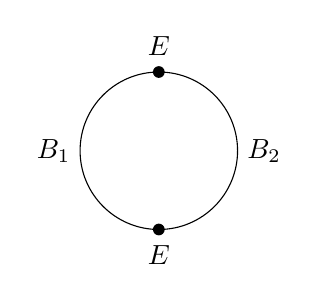
\begin{tikzpicture}[%every label/.style={green}
]
\node[fill=black, circle, label=below:$E$, inner sep=1.5pt](S) at (0,0) {};
\node[fill=black, circle, label=above:$E$, inner sep=1.5pt](N) at (0,2) {};
\draw (S) arc  (-90:90:1);
\draw (N) arc  (90:270:1);
\node[left] at (-1,1) {$B_1$};
\node[right] at (1,1) {$B_2$};
\end{tikzpicture}
\caption{Combining two balls to get a full boundary.}\label{blah3}\end{figure}

\begin{figure}
\centering
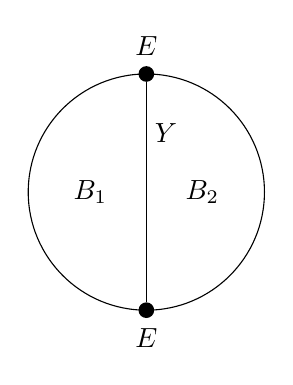
\begin{tikzpicture}[%every label/.style={green},
				x=1.5cm,y=1.5cm]
\node[fill=black, circle, label=below:$E$, inner sep=2pt](S) at (0,0) {};
\node[fill=black, circle, label=above:$E$, inner sep=2pt](N) at (0,2) {};
\draw (S) arc  (-90:90:1);
\draw (N) arc  (90:270:1);
\draw (N) -- (S);
\node[left] at (-1/4,1) {$B_1$};
\node[right] at (1/4,1) {$B_2$};
\node at (1/6,3/2)  {$Y$};
\end{tikzpicture}
\caption{From two balls to one ball.}\label{blah5}\end{figure}

\begin{figure}
\begin{equation*}
\mathfig{.23}{ncat/zz2}
\end{equation*}
\caption{A small part of $\cell(W)$.}
\label{partofJfig}
\end{figure}

\begin{figure}
%$$\mathfig{.4}{deligne/manifolds}$$
$$\mathfig{.4}{deligne/mapping-cylinders}$$
\caption{An $n$-dimensional surgery cylinder.}\label{delfig2}
\end{figure}


%% For Tables, put caption above table
%%
%% Table caption should start with a capital letter, continue with lower case
%% and not have a period at the end
%% Using @{\vrule height ?? depth ?? width0pt} in the tabular preamble will
%% keep that much space between every line in the table.

%% \begin{table}
%% \caption{Repeat length of longer allele by age of onset class}
%% \begin{tabular}{@{\vrule height 10.5pt depth4pt  width0pt}lrcccc}
%% table text
%% \end{tabular}
%% \end{table}

%% For two column figures and tables, use the following:

%% \begin{figure*}
%% \caption{Almost Sharp Front}\label{afoto}
%% \end{figure*}

%% \begin{table*}
%% \caption{Repeat length of longer allele by age of onset class}
%% \begin{tabular}{ccc}
%% table text
%% \end{tabular}
%% \end{table*}

\end{document}

